\section{Durchführung}
In Abbildung \ref{fig:01_teo} ist der Aufbau der hier verwendeten Apparatur zu sehen.
\begin{figure}
    \centering
    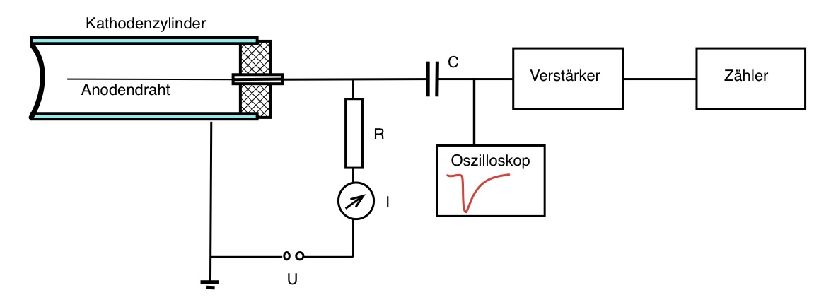
\includegraphics[width = 0.75\textwidth]{14_v703/Abbildungen/Seite 2.pdf}
    \caption{Aufbau der Messapparatur \cite{man:v703}}
    \label{fig:01_teo}
\end{figure}
Das Geiger-Müller-Zählrohr befindet sich zunächst mit einer \ce{^{204}Tl}-Probe in einer Aluminium Abschirmung.
Die restlichen Bauteile befinden sich außerhalb dieser Abschirmung.
Die Betriebsspannung wird zunächst auf die kleinste Stufe gestellt bei der der Zähler etwas zählt.
Von dort aus wird in 20 Volt Schritten die Betriebsspannung erhöht um die Zählrohrcharakteristik aufzunehmen.
Hierbei wird an dem Zähler eine Messzeit von \qty{120}{\s} eingestellt.
In dieser Messzeit finden zuverlässig mehr als \num{10000} Messungen statt, was zu einer relativen Unsicherheit von weniger als \qty{1}{\percent}führt.
Bei jeder Spannung wird auch die Stromstärke am Geiger-Müller-Zählrohr abgelesen um einen weiteren wert für die Strahlungsintensität zu generieren.

Für die zwei-Quellen-Methode wird die Betriebsspannung auf eine Spannung im ersten Drittel des Geiger-Müller-Plateaus gewählt.
In dieser Messung entspricht das einer Spannung von \qty{450}{\volt}.
In einem Zeitintervall von je \qty{120}{\s} wird die Zählrate von der einen Quelle, der anderen Quelle und den beiden Quellen zusammen gemessen.